\chapter{Event Selection}\label{chapt:event_sel}
 
This work was aiming to reconstruct the $t\bar{t}$ pair in the dilepton decay channel, or
$t\bar{t} \to W^{+}b\,W^{-}\bar{b} \to \bar{l}b\,l\bar{b}$. Thus the aim is to 
look for the event in the detector with two leptons of the different sign and two jets. The 
neutrino can't be measured directly, their presence is reflected in the non-zero transverse
missing energy $E_{T}^{miss}$. The lowest branching ratio of the dileptonic decay channel
($BR \simeq 4.8\%$) is countervailed by a a precise lepton reconstruction, which can reduce
the fraction of the background events to larger extend.

The reconstructed objects in each event (which corresponds to one bunch crossing) have to fulfill certain 
criteria to be accepted for this analysis. These criteria are chosen taking to account the physical 
result this analysis is aiming for and the technical features of the CMS detector parts.

The imperfect correspondence of the simulation model to the real data has to be additionally 
corrected. The differences in the efficiencies of certain procedures in data and simulation 
are corrected by applying \textit{Scale Factors}, $SF = \frac{\epsilon_{data}}{\epsilon_{MC}}$, 
on the MC distributions. Here $\epsilon_{data}$ is the efficiency determined in the experimental 
data and $\epsilon_{MC}$ is the efficiency from simulation. 

This chapter gives an overview of the $t\bar{t}$ event selection. The 
procedures are based on the CMS Top-Quark-Physics-Analysis group recommendations \cite{TopPAGreco}.
The full chain of event selection are described. 
Resulting event yields are represented in the control distributions, showing the data, simulated signal and backgrounds.

\section{Background Sources}\label{sec:bg_intro}

Not all of these events which have two leptons and two jets in the final state are the \textbf{signal events} 
originating from the $t\bar{t}$ system decay in dileptonic channel. The final state, which can be 
misidentified as $t\bar{t}$, may arise from a different process, called \textit{background}
for the specific measurement. In this analysis the background rates are estimated from the simulation.
The following background processes are discussed in frames of this analysis:

\begin{itemize}
 \item $t\bar{t}\rightarrow$other. This background source includes the other $t\bar{t}$ decay modes (see sec. \ref{ssec:tdecay}).
 \item single top production, which was simulated using \Powheg + \PYTHIA;
 \item Drell-Yan process, which was generated utilizing \PYTHIA. It can be mistreated as $t\bar{t}$ signal, as it also has a dileptonic
 final state signature. However, only the same flavour leptons are produced in Drell-Yan processes. Therefore, the fraction of these
 background events in the $e\mu$ final state is small;
 \item diboson production, simulated using \PYTHIA. These events also have the leptonic final state and may be picked as a $t\bar{t}$
 candidate;
 \item $Z/\gamma^{*} \rightarrow \tau\tau$ production, which was generated using \PYTHIA. Here the $\tau$-leptons decay further
 to $e$, $\mu$ and neutrinos;
 \item $Z/\gamma^{*} \rightarrow ee/\mu\mu$ production, generated using \PYTHIA;
 \item associated $t\bar{t}\;+\; W/Z/\gamma$ production, simulated in \MG + \PYTHIA;
 \item associated $W\;+\;jets$ production, generated using \MG + \PYTHIA;
 \item QCD multijet processes, generated in \PYTHIA.
\end{itemize}

To be able to compare these generated background samples, they were normalized to the data integrated luminosity of 19.7 fb$^{-1}$ and
to their production cross sections\cite{TWikiXSec}.

The selection, which will be introduced in this section, is aiming to distinguish the $t\bar{t}$ events
from the background processes exploiting physical features of each process.

\section{Good Runs}

For the work presented in this thesis the following CMS data samples were used:

\begin{center}\label{tab:samples}
  \begin{tabular}{| c c c |}
    \hline
    \textbf{Samples} & \textbf{Events} & \textbf{Run Range} \\ \hline
    /MuEG/Run2012A-22Jan2013-v1/AOD & 2.5M & 190456 - 193621 \\ 
    /MuEG/Run2012B-22Jan2013-v1/AOD & 15M & 193834 - 196531 \\
    /MuEG/Run2012C-22Jan2013-v1/AOD & 21M & 198022 - 203742 \\
    /MuEG/Run2012D-22Jan2013-v1/AOD & 22M & 203777 -  208686 \\
    \hline
  \end{tabular}
\end{center}

Only the good runs from the LHC certified good run list\cite{JSON} are selected for the analysis out of these data sets.

\section{$t\bar{t}$ Event Selection and Correction}\label{sec:sel}

Various selection criteria and related scale factors are presented in this section.

The results of the selection are presented in the control distributions. These plots show the comparison between the yields in the experimental data and the simulated MC samples.
The various background sources are also presented separately in the distributions. The simulated yields are additionally scaled to the data luminosity of 19.7\;$fb^{-1}$.
All the plots include the statistical uncertainties only.

All the selection requirements are summarized as follows:

\begin{itemize}
 \item [--] \textbf{Trigger selection}: The events have to be accepted by the HLT (see section \ref{sec:trig}) dilepton triggers, which require the presents of two leptons, electrons or muons, with
 minimum transverse momentum of 17 GeV and 8 GeV.
 
 The Scale Factors connected to the trigger selection were applied on the MC double-differentially in bins of the two leptons rapidities. 
 %%%% 
 \item [--] \textbf{Beam scrapping}: Accept only events with maximum 10 reconstructed tracks, or more then 10 in case at least quarter of them has high quality of reconstruction.
 %%%%
 \item [--] \textbf{Calorimeter noise removal}: Event with anomalous calorimeter noise are removed.
 %%%%
 \item [--] \textbf{Vertex requirement}: Events with at least one "good" primary vertex are selected.
 This means that the number of associated tracks should be larger then 4 and a vertex should be positioned centrally in the detector
 \footnote{Only the events with the vertex position $|z| < \textrm{24 cm}$ and $|\rho| < \textrm{2 cm}$ are accepted. All the coordinates
 are given with respect to the CMS coordinate system (see sec.\ref{sec:CMS})}. Only the ``hardest vertex'' 
 (with the highest sum of the $p_{T}^{2}$ of the assigned tracks) is taken for the analysis. 
 \\
 An additional weight correction depending on the event vertex multiplicity is applied on the MC. 
 The distributions presented in the figure \ref{fig:PUweight} show how the agreement
 between the experimental and simulated data improves after this reweighting is implemented.
 
 \begin{figure}[h]
 \centering
 \begin{subfigure}
   \centering
   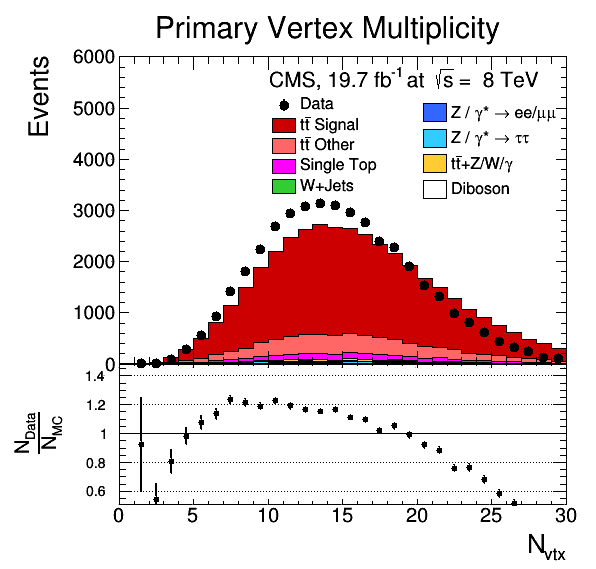
\includegraphics[width=0.49\textwidth]{04_event_reconstruction/plots/vertex_mult_noPUw.png}
 \end{subfigure}
 \begin{subfigure}
   \centering
   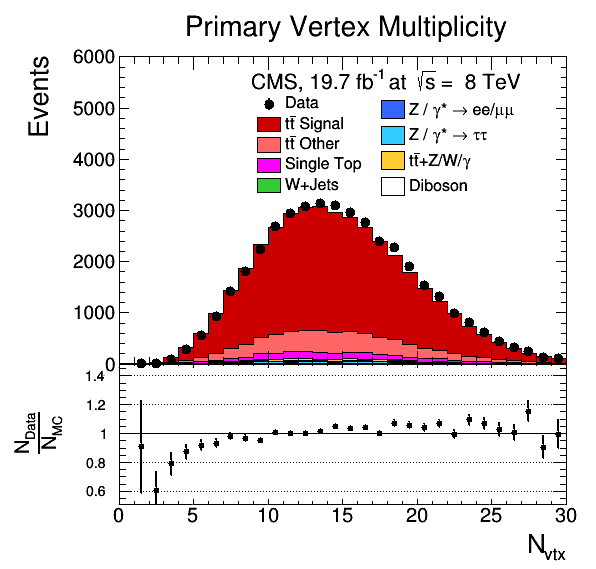
\includegraphics[width=0.49\textwidth]{04_event_reconstruction/plots/vertex_mult_PUw.png}
 \end{subfigure}
 \caption{The vertex multiplicity control distribution before (left) and after (right) the vertex correction reweighing after the full event selection.
 Black dots represent the experimental data and the colored histograms are the MC simulation divided into signal and backgrounds contributions.
 The bottom plots represent the ratio between experimental and simulated data rates.}
 \label{fig:PUweight}
 \end{figure}
 
 %%%%%
 \item [--] \textbf{Lepton isolation}: All the leptons in the event have to be isolated with $I_{rel}\leq 0.15$ in a cone of $\Delta R = \sqrt{\Delta\eta^{2} + \Delta\phi^{2}} = 0.3$ 
 around the lepton track, where $I_{rel}$ is the relative isolation defined as:
  \begin{equation}\label{eq:Iso}
   I_{rel} = \frac{\sum E_{Tracker} + \sum E_{ECAL} + \sum E_{HCAL}}{p_{T}(l)}
  \end{equation}
 
 As it is shown in the figure \ref{fig:PFIso}, the lepton isolation requirement cuts on the events which dominated by the QCD background.

 \begin{figure}[h]
 \centering
 \begin{subfigure}
   \centering
   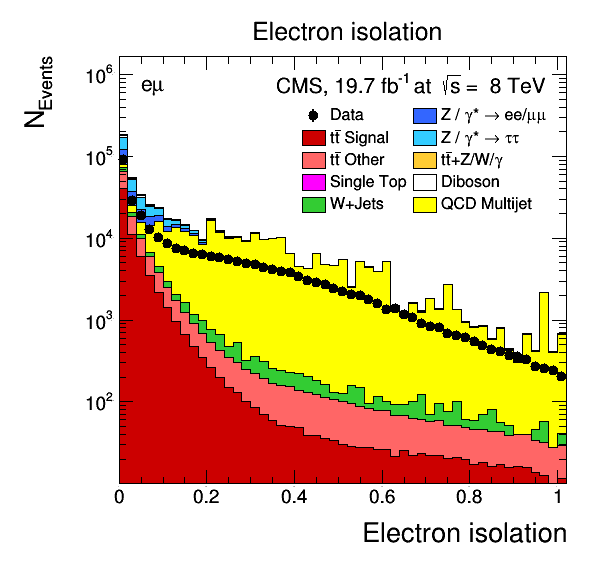
\includegraphics[width=0.49\textwidth]{04_event_reconstruction/plots/PF_e_Iso.png}
 \end{subfigure}
 \begin{subfigure}
   \centering
   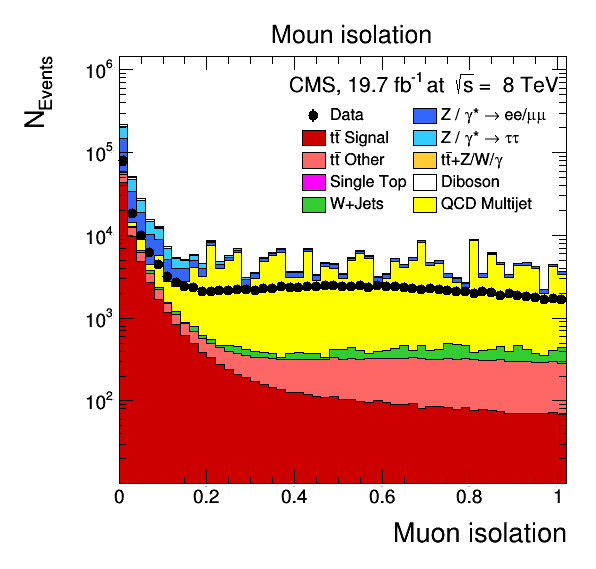
\includegraphics[width=0.49\textwidth]{04_event_reconstruction/plots/PF_mu_Iso.png}
 \end{subfigure}
 \caption{The electron (left) and muon (right) relative isolation $I_{rel}$ (\ref{eq:Iso}) control distributions displaying the experimental data points
 and simulated distributions of signal and different background after the trigger selection. The vertical dashed lines show the isolation cut value.}
 \label{fig:PFIso}
 \end{figure}
 
 The efficiencies of the lepton isolation were determined using \textbf{tag and probe} method \cite{TWikiTP}. The corresponding scale factors are applied on the
 simulation level in bins of $p_{T}$ and $\eta$ of lepton separately for electrons and for muons.
 %%%%%
 \item [--] \textbf{Lepton pair selection}: An event has to contain at least two opposite signed leptons (electron-muon pair) with $p_{T} > 20 \; \textrm{GeV}$ and $|\eta| < 2.4$.
 The invariant mass of the system of the leading $p_{T}$ electron and muon has to be more than 20 GeV, otherwise the event is rejected. 
 %%%%%
 \item [--] \textbf{Jets selection}: Events which contain at least two jets with $p_{T} > 30$ GeV and $|\eta| \leq 2.4$ are accepted. It is natural to expect
 that events with less than two jets will be dominated by Drell-Yan background as the leading order Drell-Yan process does not contain jets in the final state. This is also 
 reflected by the jet multiplicity distribution (Fig. \ref{fig:jetMultiSel}). 
 
 \begin{figure}[h]
  \centering
  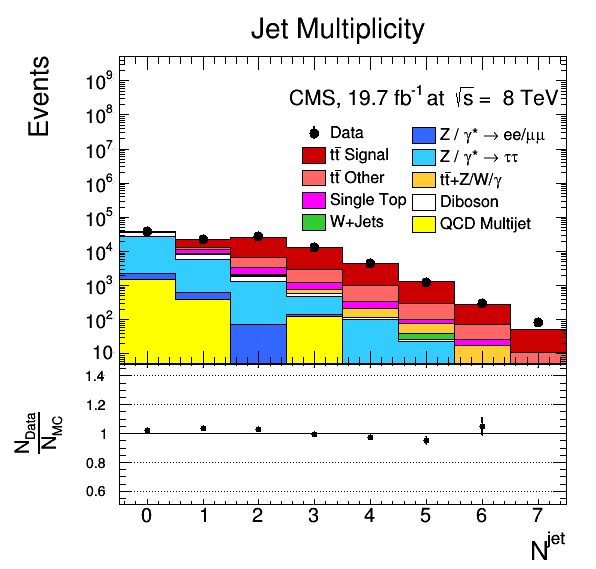
\includegraphics[width=0.6\textwidth]{04_event_reconstruction/plots/JetMulti.png}
  \caption{The control distribution of the jet multiplicity in the events after the trigger and lepton selection. The experimental data points
  and simulated distributions of signal and different backgrounds are plotted. The error bars of the data points
 correspond to the statistical uncertainties of the measurement. The bottom plots represent the data-to-MC yield ratio distributions.}
  \label{fig:jetMultiSel}
 \end{figure}
 
%  In the figure \ref{fig:mllJetSel} the dilepton mass before and after jet selection is shown, demonstrating a sizable background (especially Drell-Yan) fraction suppression power
%  of the cuts implemented in this selection step.
%  
%  \begin{figure}[h]
%  \centering
%  \begin{subfigure}
%    \centering
%    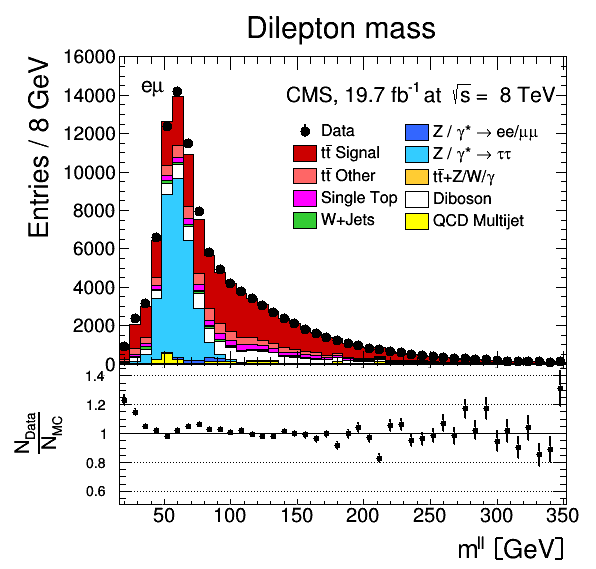
\includegraphics[width=0.49\textwidth]{04_event_reconstruction/plots/mll_step4.png}
%  \end{subfigure}
%  \begin{subfigure}
%    \centering
%    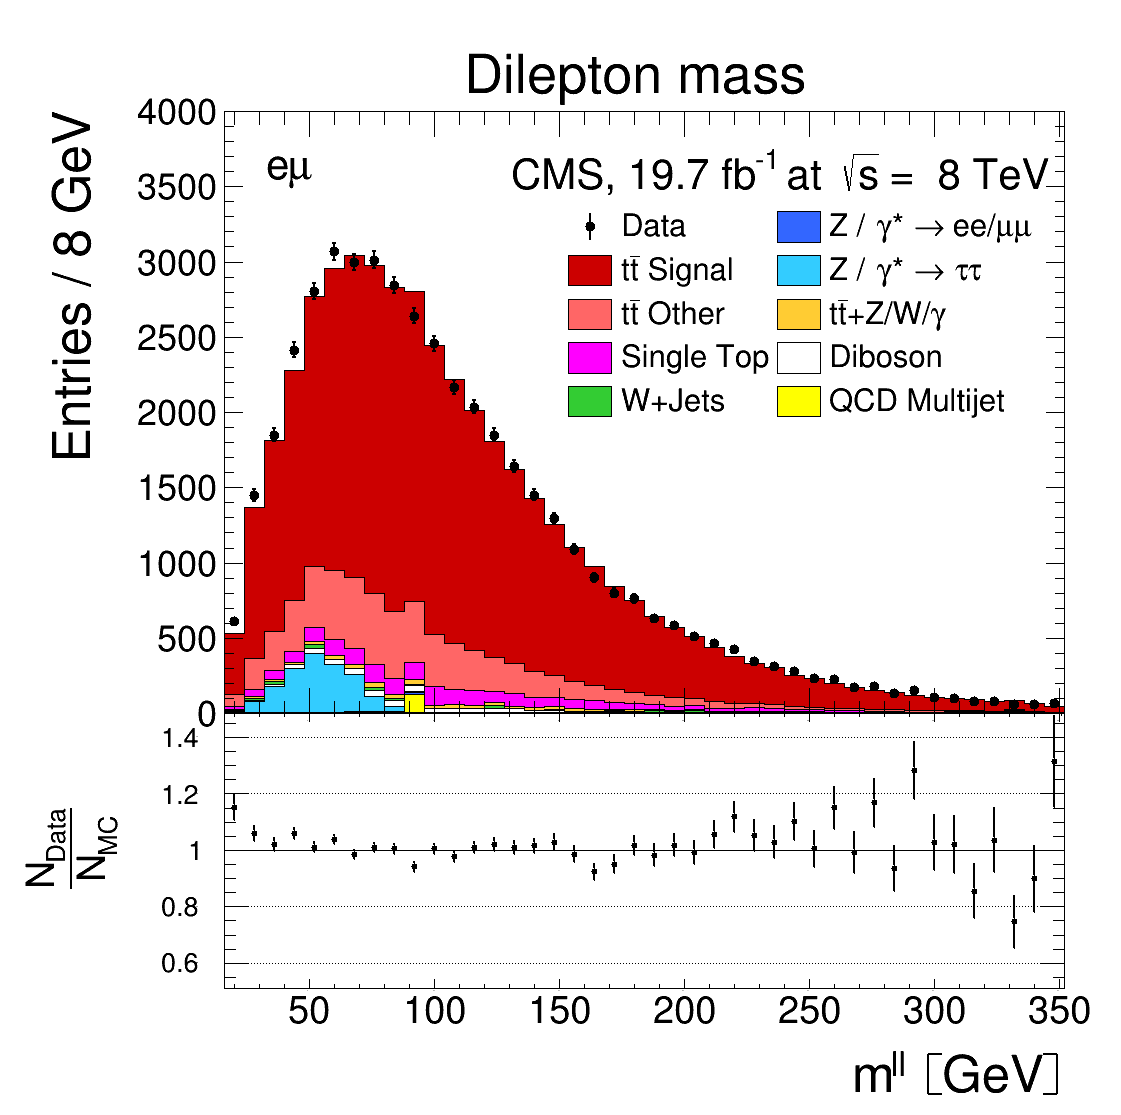
\includegraphics[width=0.49\textwidth]{04_event_reconstruction/plots/mll_step5.png}
%  \end{subfigure}
%  \caption{The control distribution of the dilepton mass in the events after the trigger and lepton selection (left) and after trigger, lepton and jet selection (right). 
%  The experimental data points and simulated distributions of signal and different background are plotted.}
%  \label{fig:mllJetSel}
%  \end{figure}
 %
 \item [--] \textbf{$b$-jets selection}: An event has to contain at least one jet, tagged as originating from the $b$-quark with the b-tagging probability according to the CSVL (sec. \ref{ssec:bTag}). The multiplicity of the $b$-tagged
 jets is presented in the figure \ref{fig:bjetMultiSel} which shows that cutting out the events with no $b$-tagged jets should remove a sizable background fraction. Indeed, the figure \ref{fig:mllbJetSel} presenting
 the dilepton mass before and after the $b$-jets selection shows this background reduction.
 
 \begin{figure}[h]
  \centering
  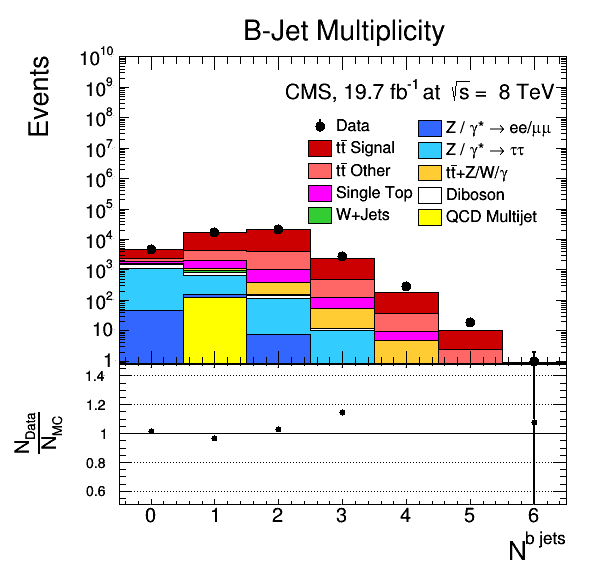
\includegraphics[width=0.6\textwidth]{04_event_reconstruction/plots/bJetMulti.png}
  \caption{The control distribution of the $b$-jet multiplicity in the events after the trigger, lepton and jet selection. The experimental data points
  and simulated distributions of signal and different background are plotted. The error bars of the data points
  correspond to the statistical uncertainties of the measurement. The bottom plots represent the data-to-MC yield ratio distributions.}
  \label{fig:bjetMultiSel}
  \end{figure}
  
 \begin{figure}[h]
 \centering
 \begin{subfigure}
   \centering
   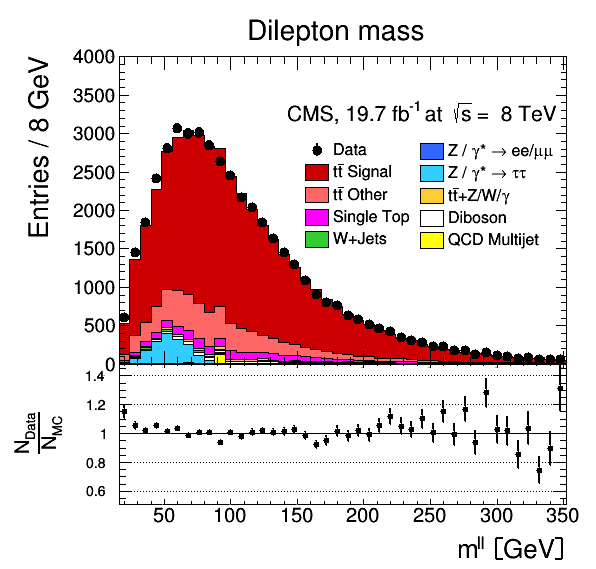
\includegraphics[width=0.49\textwidth]{04_event_reconstruction/plots/mll_step6.png}
 \end{subfigure}
 \begin{subfigure}
   \centering
   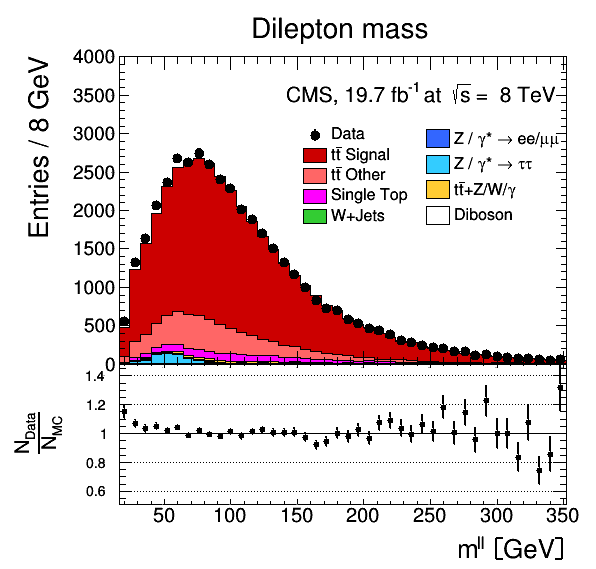
\includegraphics[width=0.50\textwidth]{04_event_reconstruction/plots/mll_step7.png}
 \end{subfigure}
 \caption{The control distribution of the dilepton mass in the events after the trigger, lepton and jet selection (left) and after applying in addition the $b$-jet selection (right). 
 The experimental data points and simulated distributions of signal and different background are plotted. The error bars of the data points
 correspond to the statistical uncertainties of the measurement. The bottom plots represent the data-to-MC yield ratio distributions.}
 \label{fig:mllbJetSel}
 \end{figure}
 
 The scale factors corresponding to the $b$-tagging procedure were applied on the MC improving much the agreement between data and simulation. This effect can be seen in the 
 figure \ref{fig:bTagDiscr}, which presents the CSV discriminator distribution before and after the $b$-tagging SF reweighing. The data-to-MC ratio plots are getting closer to one with
 applying the SFs.
 
 \begin{figure}[h]
 \centering
 \begin{subfigure}
   \centering
   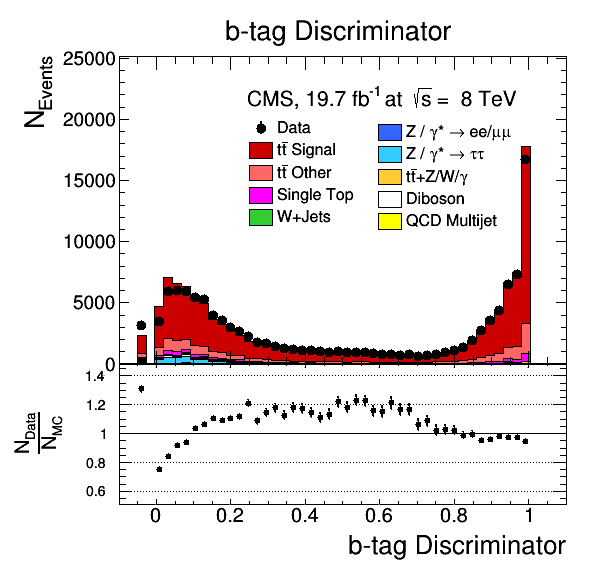
\includegraphics[width=0.49\textwidth]{04_event_reconstruction/plots/bTagDiscr_step6.png}
 \end{subfigure}
 \begin{subfigure}
   \centering
   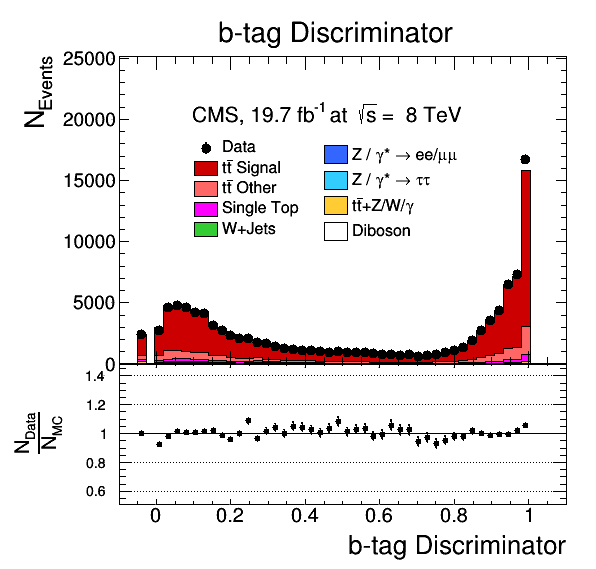
\includegraphics[width=0.49\textwidth]{04_event_reconstruction/plots/bTagDiscr_step7.png}
 \end{subfigure}
 \caption{The control distribution of the $b$-tag discriminator in the events after the full even selection (\ref{sec:sel}) not applying the $b$-tag Scale Factors (left)
 and after applying the $b$-tag Scale Factors (right). The experimental data points and simulated distributions of signal and different background are plotted.
 The error bars of the data points correspond to the statistical uncertainties of the measurement.
 The bottom plots represent the data-to-MC yield ratio distributions.}
 \label{fig:bTagDiscr}
 \end{figure}
 %
 \end{itemize}

The applied selection criteria dramatically reduced the fraction of background events.

\section{Control Distributions}

The results of the reconstruction and selection described above can be illustrated by control distributions of the objects which are reconstructed for the $t\bar{t}$
final state definition.

The figure \ref{fig:CPetaptLep} shows the lepton $\eta$ and $p_{T}$. An overall reasonable agreement between the data and simulation shapes is observed in all $\eta$ regions
and $p_{T}$'s. The control distribution of the mass of the dilepton (electron-muon) system is shown in figure \ref{fig:CPmll}. The simulation and experimental data
agree well within the statistical uncertainties except for the first bin where data are higher than simulation.

 \begin{figure}[h]
 \centering
 \begin{subfigure}
   \centering
   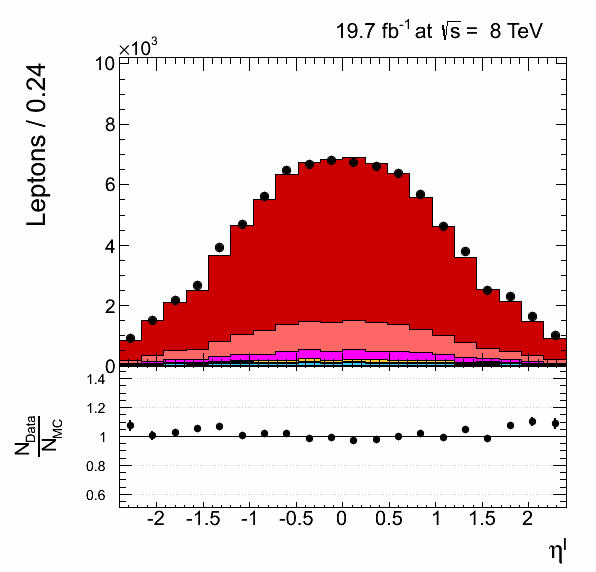
\includegraphics[width=0.49\textwidth]{04_event_reconstruction/plots/basic_lepton_eta_step7.png}
 \end{subfigure}
 \begin{subfigure}
   \centering
   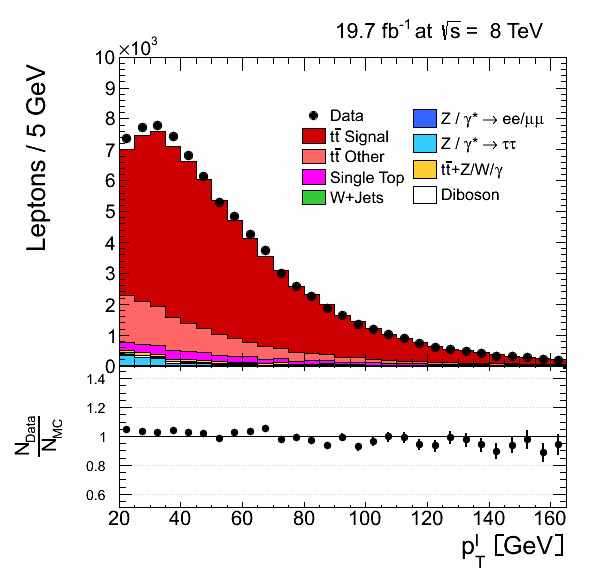
\includegraphics[width=0.49\textwidth]{04_event_reconstruction/plots/basic_lepton_pt_step7.png}
 \end{subfigure}
 \caption{The control distribution of lepton $\eta$ (left) and lepton $p_{T}$ (right) in the events after the whole event selection (\ref{sec:sel}). 
 The experimental data points and simulated distributions of signal and different background are plotted. The error bars of the data points
 correspond to the statistical uncertainties of the measurement. The bottom plots represent the data-to-MC yield ratio distributions. 
 Each distribution has two entries per event - for the electron and for the muon.}
 \label{fig:CPetaptLep}
 \end{figure}
 
 \begin{figure}[h]
  \centering
  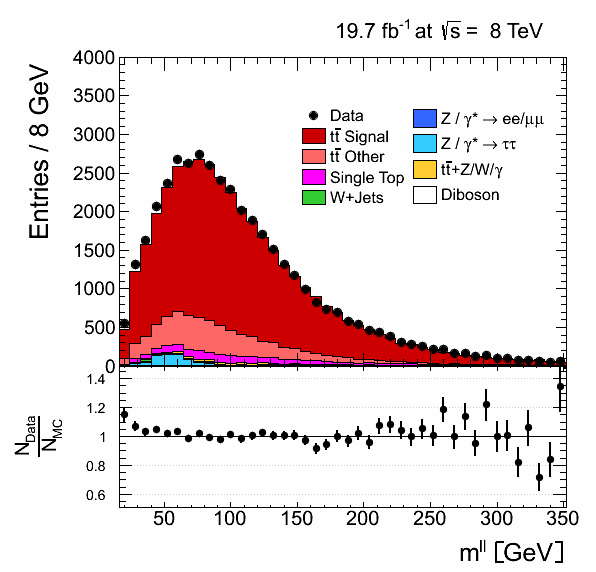
\includegraphics[width=0.6\textwidth]{04_event_reconstruction/plots/basic_dilepton_mass_step7.png}
  \caption{The control distribution of the mass of the electron-muon system in the events after the whole \ref{sec:sel} selection. 
  The experimental data points and simulated distributions of signal and different background are plotted. The jets $p_{T}$ and multiplicity 
  distributions are presented in the logarithmic scale. The error bars of the data points
  correspond to the statistical uncertainties of the measurement. The bottom plots represent the data-to-MC yield ratio distributions.}
  \label{fig:CPmll}
 \end{figure}
 
The kinematics of the reconstructed and selected jets is presented in the figure \ref{fig:CPjetskin} which shows the control distributions for the
jets $\eta$, $p_{T}$ and the jet multiplicity in the events. The simulation describes better the central rapidity ranges. For the jet multiplicities
smaller than 5 a good agreement between experimental data and MC is observed.
 
 \begin{figure}[h]
 \centering
 \begin{subfigure}
   \centering
   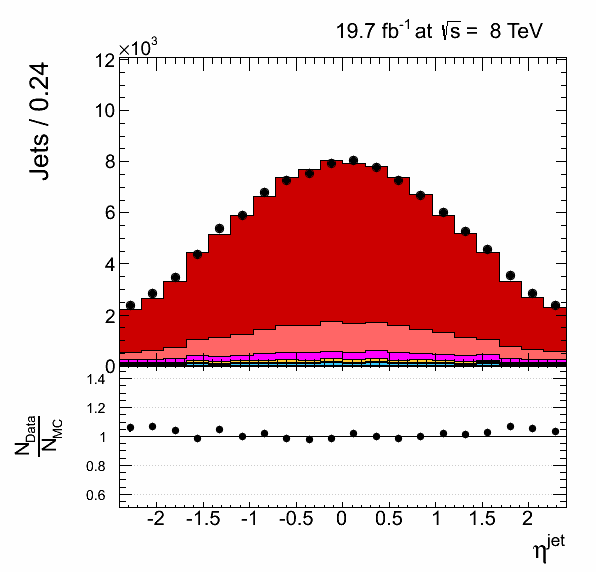
\includegraphics[width=0.49\textwidth]{04_event_reconstruction/plots/basic_jet_eta_step7.png}
 \end{subfigure}
 \begin{subfigure}
   \centering
   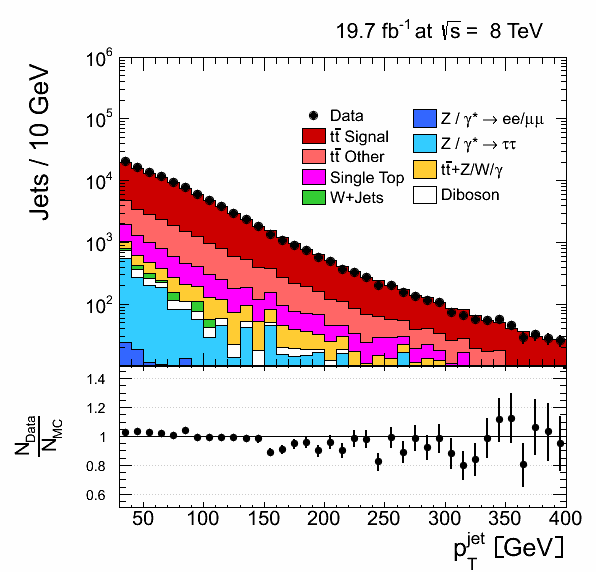
\includegraphics[width=0.49\textwidth]{04_event_reconstruction/plots/basic_jet_pt_step7.png}
 \end{subfigure}
  \begin{subfigure}
   \centering
   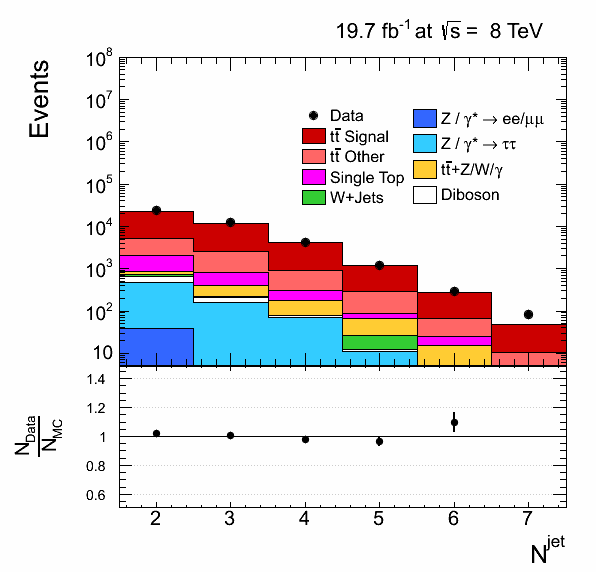
\includegraphics[width=0.49\textwidth]{04_event_reconstruction/plots/basic_jet_multiplicity_step7.png}
 \end{subfigure}
 \caption{The control distribution of the jet $\eta$ (top left) and jet $p_{T}$ (top right) and jet multiplicity in the events 
 after the whole \ref{sec:sel} selection. The experimental data with the error bars corresponding to the statistical uncertainties
 and simulated distributions of signal and different background are plotted. The bottom plots represent the data-to-MC yield ratio distributions. 
 The top distributions have multiple entries per event, corresponding to all reconstructed jets.}
 \label{fig:CPjetskin}
 \end{figure}
 
The multiplicity for the $b$-tagged jets is presented in figure \ref{fig:CPbJetMult} which shows a good agreement for the multiplicities smaller than 4.

 \begin{figure}[h]
  \centering
  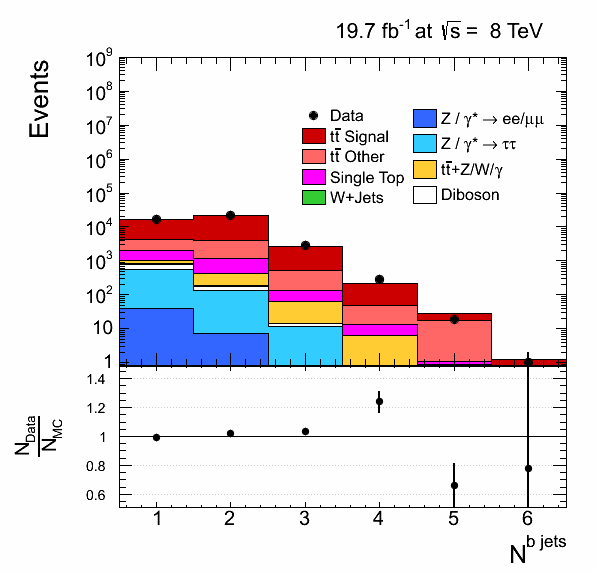
\includegraphics[width=0.6\textwidth]{04_event_reconstruction/plots/basic_bjet_multiplicity_step7.png}
  \caption{The control distribution of the $b$-tagged jets multiplicities in the events after the whole \ref{sec:sel} selection. 
  The experimental data points and simulated distributions of signal and different background are plotted in the logarithmic scales. 
  The error bars of the data points correspond to the statistical uncertainties of the measurement. 
  The bottom plots represent the data-to-MC yield ratio distributions.}
  \label{fig:CPbJetMult}
 \end{figure}
 
The control distributions are signal dominated which shows a good performance of the criteria for the $t\bar{t}$ final state selection.



